
\section{Rozwiązywanie zadań z  pomocą MES}
\label{sec:rozwiazwyanie_zadan}

W wytrzymałości materiałów poszukujemy zwykle sił działających w podporach konstrukcji i naprężeń wewnątrz jej konkretnych elementów. Innym podejściem jest znalezienie pola przemieszczeń dla każdego punktu konstrukcji.  W jednym i drugim przypadku znalezienie niewiadomych jest osiągalne wyłącznie dla mało skomplikowanych konstrukcji.

Metoda elementów skończonych bierze swoją nazwę od wydzielanych fragmentów konstrukcji, które są właśnie elementami skończonymi. Elementy tworzymy na siatce węzłów, które są punktami wewnątrz lub na brzegach konstrukji. Węzły są także punktami wspólnymi sąsiadujących elementów. Rozwiązanie opiera się na znalezieniu przemieszczenia węzłów i na tej podstawie obliczenia rozwiązania we wszystkich punktach wewnątrz elementów. Kolejne etapy rozwiązywania zadania za pomocą MES przedstawione są poniżej. Rysnuek \ref{fig:MES_przyklad} przedstawia przykład obiektu, który został zdyskretyzowany za pomocą elementów skończonych.

\vspace{5 mm}

\begin{enumerate}
  \item Generacja siatki węzłów.
  \item Budowa elementów skończonych na stworzonej siatce.
  \item Wyznaczanie macierzy mas i sztywności dla każdego elementu (macierze lokalne).
  \item Agregacja macierzy mas  i sztywności dla całej konstrukcji (macierze globalne).
  \item Wprowadzenie wektora obciążeń.
  \item Wprowadzenie warunków brzegowych. Mogą to być siły czynne (modyfikacja wektora obciążeń), naprężenia początkowe czy przemieszczenia wskazanych węzłów.
  \item Rozwiązanie wyznaczonego liniowego równania różniczkowego \( M \ddot x + Kx = F \) - znalezienie przemieszczeń węzłów.
  \item Wyznacznie odkształceń i naprężeń.
  \item Wyznaczenie reakcji w podporach (węzłach, dla których założono przemieszczenie)
\end{enumerate}

\vspace{5 mm}

\begin{figure}[h]
\centering
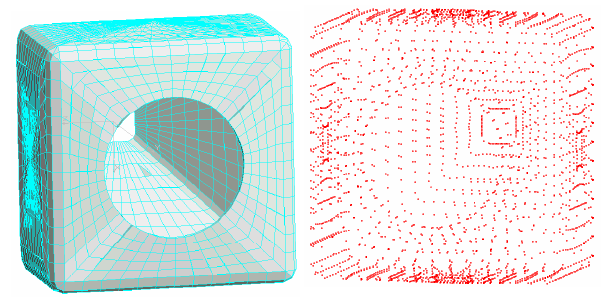
\includegraphics[width=10cm]{Zdjecia/3/MES_przyklad}
\caption{Przykład dsykretyzacji obiektu za pomocą elementów skończonych \cite{bartek_srodka}}
\label{fig:MES_przyklad}
\end{figure}





















